\documentclass[11pt, oneside]{article}   	% use "amsart" instead of "article" for AMSLaTeX format
\usepackage{geometry}                		% See geometry.pdf to learn the layout options. There are lots.
\geometry{letterpaper}                   		% ... or a4paper or a5paper or ... 
%\geometry{landscape}                		% Activate for rotated page geometry
%\usepackage[parfill]{parskip}    		% Activate to begin paragraphs with an empty line rather than an indent
\usepackage{graphicx}				% Use pdf, png, jpg, or eps§ with pdflatex; use eps in DVI mode
								% TeX will automatically convert eps --> pdf in pdflatex		
\usepackage{amssymb}
\usepackage{amsmath}
\usepackage[french]{babel}
\usepackage[utf8]{inputenc}
\usepackage[T1]{fontenc}

%SetFonts

%SetFonts


\title{Brief Article}
\author{BOUJNOUNI Fatine, AFCHAR HERAVI MOGHADAM Darius, TOULEMONT Matthieu}
%\date{}							% Activate to display a given date or no date

\begin{document}
\maketitle
\section{Introduction}
L'objectif de notre projet est la mise en correspondance automatique de textes en langues différentes sans connaissances préalables. Dans notre projet, nous prenons en considération les langues européennes ( Français, Anglais, Espagnole, Allemand..), et nous supposons qu'on a des textes suffisamment longs où on peut trouver des mots avec des traductions " faciles " dans le texte traduit.

Nous avons fait une traduction mot à mot en utilisant les algorithmes dynamiques de dilatation temporelle ( Dynamic Time Warping Algorithms).
Ensuite, nous avons essayé de faire une classification morphologique des mots qui apparaissent dans les deux textes à travers la méthode de " Goldsmith" et la méthode " Patricia Trie et nouvelle heuristique " et nous communiquons nos résultats à travers une interface graphique.


%\subsection{}
\section{Architecture choisie}
\subsection{Diagramme de package}
Ce diagramme de package décrit les principales fonctionnalités de notre projet et les principales parties sur lesquelles on a travaillé.
\begin{figure}[h!]
\centering
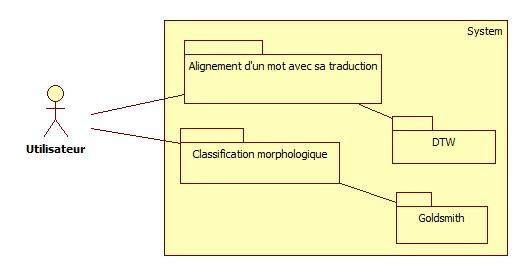
\includegraphics[width = 260pt]{diag_pack.jpg}
\end{figure}

\subsection{Interface graphique}
Pour notre interface graphique on a utilisé un modèle MVC ( Modèle-Vue-contrôleur). Le diagramme de classes suivant détaille cette architecture :

\begin{figure}[h!]
\centering
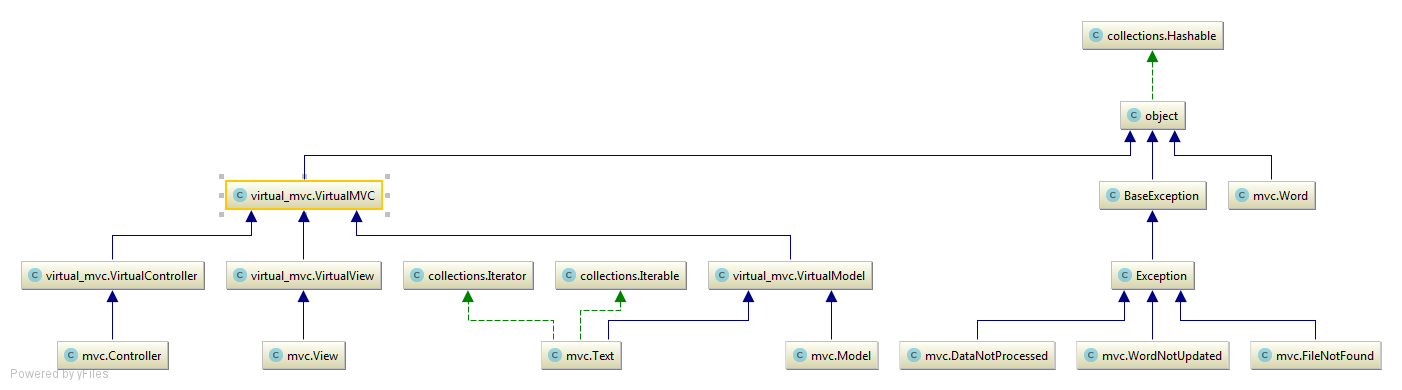
\includegraphics[width = 500pt]{mvc.png}
\end{figure}

Et ce diagramme détaille les différentes classes qui constituent notre fenêtre:

\begin{figure}[h!]
\centering
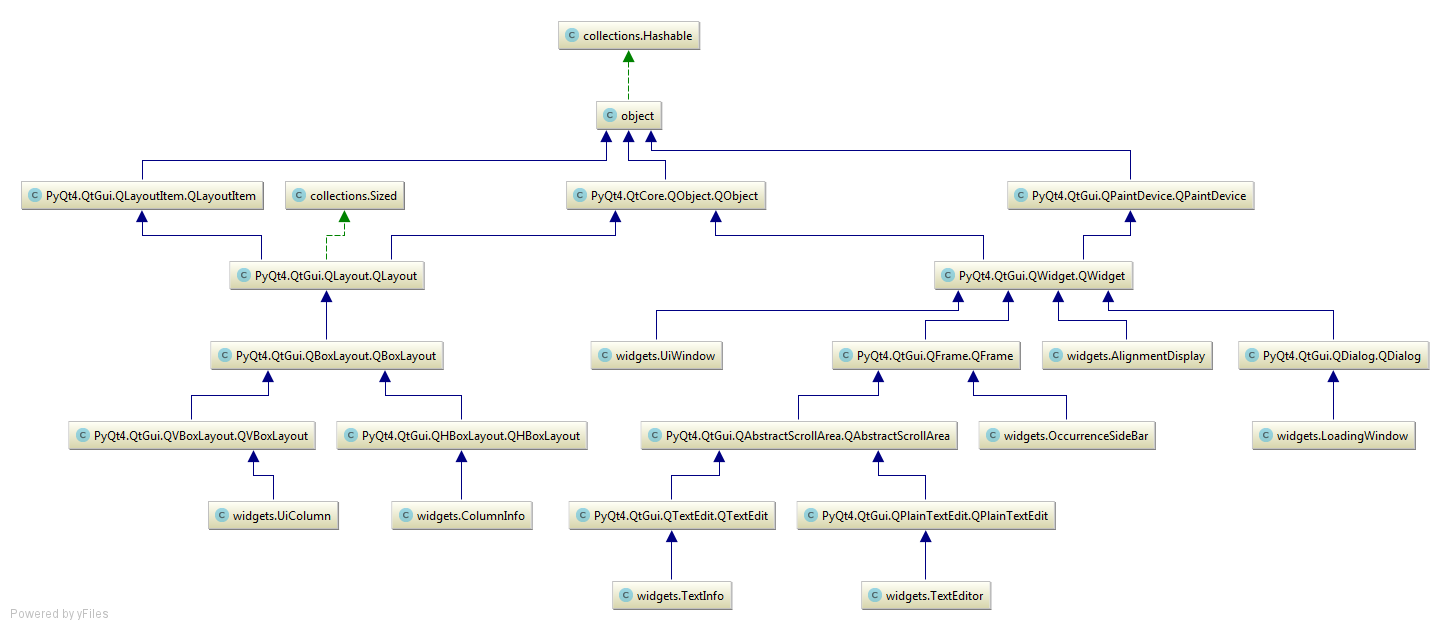
\includegraphics[width = 500pt]{widget.png}
\end{figure}


\section{Alignement de mot}
Il existe plusieurs systèmes d'alignement de textes qui se basent sur les formes de similitude graphique entre un texte et sa traduction. Comme l'alignement par cognats ( lexicaux ou de ponctuation). L'idée de base pour l'alignement par cognats lexicaux est l'exploitation de la similitude graphique entre un mot et sa traduction, surtout lorsqu'il s'agit de noms propres ou de mots d'origine grecque ou latine et qui s'écrivent de la même manière dans les langues européennes. 

L'alignement qu'on a effectué se base sur les algorithmes dynamiques de dilatation temporelle, qui sont basés sur la distribution dans le texte entier d'un mot et de sa traduction. L'idée derrière cette approche, est que le signal du mot à traduire dans le corpus à aligner ressemble à celui de sa traduction dans la langue cible.

La méthode fonctionne de la manière suivante: 

- Traitement des textes à aligner dans la mémoire.

- On calcule pour chaque mot son vecteur de récence: on représente la distance ( en nombre de caractères ) entre chaque apparition du mot.

- On normalise ce vecteurs en passant à des fractions du texte entier.

- La similitude des signaux ( qui apparaissent sur le diagramme des vecteurs de récences ) est ce qui determine les paires de mots qu'on pourra aligner.

\section{Interface}
\begin{figure}[h!]
\centering
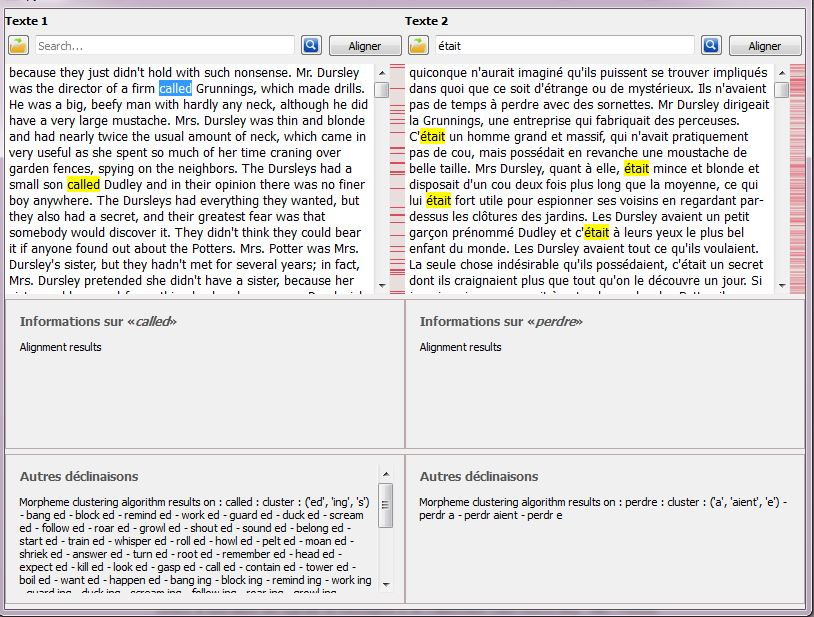
\includegraphics[width = 400pt]{interface.jpg}
\end{figure}

L’interface est divisée en deux colonnes. Chaque colonne est réservée pour l’ouverture et l’affichage d’un des deux textes.

On a aussi sur chaque colonne une partie en bas où s’affichent les résultats de la classification morphologique de chaque mot sélectionné.
On suppose qu’on peut effectuer l’alignement à partir des deux textes. D’où la présence du bouton « Aligner » sur les deux côtés.
On dispose aussi des boutons qui nous permettent d’ouvrir les textes et chercher un mot sur le texte.


\subsection{Fonctionnalités de l'interface}
-	Permet d’ouvrir deux textes.

 
-	Permet de chercher un mot et ses occurrences grâce à la barre de recherche.

-	Permet d’afficher en couleur jaune toutes les occurrences d’un mot sélectionné. 

-	Permet de se déplacer entre les occurrences d’un mot grâce aux surlignages en rouge qui se trouvent sur la barre de défilement. 

-	 Permet d’aligner un mot dans un texte et sa traduction dans l’autre texte.

-	Permet d’afficher les résultats de la classification morphologique.

\section{Classification morphologique}
Après avoir effectué l'alignement des mots, nous avons voulu tenter de classifier les mots selon leur morphologie. Une première approche fut d'utiliser l'algorithme défini par John Goldsmith et al dans leur article de 2001 : http://www.aclweb.org/anthology/J01-2001. Puis après des premiers résultats et un échange de mails avec Mr Goldsmith nous avons décidé de changer de méthode, en majeur partie à cause du temps qu'il nous restait pour trouver une solution.

\subsection{Première méthode : Goldsmith}
L'idée principale de cette méthode est de créer un ensemble de segmentation des mots en radicaux et en suffixes:
\begin{equation}
mot = \{(radical_{i}, suffixe_{i})\}
\end{equation}

Une fois cette segmentation effectuée, on veut former ce qu'on appelle des signatures défini comme suit : 
\begin{equation}
signature = \{radical_{i}, radical_{j}...\} <-> \{suffixe_{k}, suffixe_{m}\}
\end{equation}
tel que $\forall$ $i$, $k$  $radical_{i} + suffixe_{k}$ est un mot dans le texte. Chaque mot doit être encoder dans une seule signature. 

Les premières segmentations nous permettent de créer un premier ensemble de signatures parmi lesquelles nous devons bien sûr en éliminer la plus part. Pour cela les auteurs de l'article utilisent la MDL ou Minimum Description Length définit par Rissanen. Ils définissent donc, pour chacun des objets, une longueur de compression, et vont chercher à minimiser la somme de toutes ces longueurs. Ne précisant pas comment ils effectuent cette minimisation nous avons premièrement choisi de maximiser ce que les auteurs appellent l'information mutuelle pondérée d'un suffixe : 

\begin{equation}
\frac{[suffixe]}{[kgram]}*log(\frac{[suffixe]}{\prod_{lettre\in suffixe}^{}[letter]}
\end{equation}

où $[suffixe]$ est le nombre de fois où le suffixe apparait dans le texte en tant que suffixe. En plus de cela nous avons cherché à maximiser pour chaque signature le produit suivant : 

\begin{equation}
log(|radical|)*log(|suffixe|)
\end{equation}

où $|suffixe|$ est le nombre de suffixe dans la signature. Ceci dans l'idée que nous voulions éviter au maximum les signatures ne contenant qu'un seul suffixe ou un seul radical puisque qu'elle n'apporte pas d'informations générales sur la langue du texte étudié.

Après un mois et demi sur cette méthode nos résultats n'étaient pas encourageant, nous avons décidé d'envoyer un mail à Mr Goldsmith pour plus de détails sur la méthode à employer. Il nous a grandement aidé, conforté dans nos résultats et nous a conseillé de changer d'estimateur et d'utiliser plutôt la MDL de Rissanen. Manquant de temps pour se plonger dans cette méthode et la mettre en place nous avons choisi de changer d'estimateurs et de méthode d'agrégation des signatures. 

\subsection{Seconde méthode : Patricia Trie et nouvelle heuristique}

Ici nous avons commencé par encoder le texte dans un Patricia Trie. 

\begin{figure}[!h]
\centering
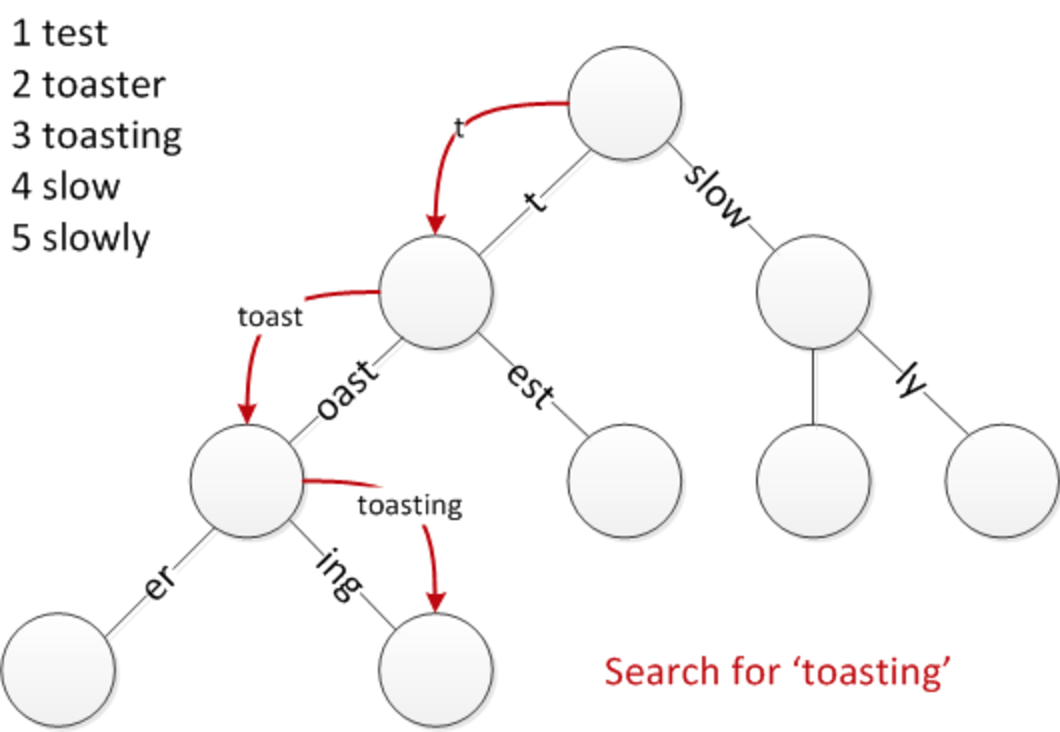
\includegraphics[width = 200pt]{patricia_trie.png}
\caption{Cette photo provient de la page wikipedia sur les patricia trie}
\end{figure}

Une fois cet arbre construit, on peut avoir accès à ses feuilles dont on est sûr qu'elles constituent des suffixes. De plus en parcourant l'arbre et en s'arrêtant dès qu'on tombe sur un mot du texte on obtient une première décomposition du mot et de tous ceux qui suivent dans l'arbre. En bref, l'utilisation d'un patricia trie nous permet d'obtenir un premier sous ensembles de suffixes et une première segmentation pour chaque mot. Pour construire cet arbre nous avons bénéficié du code de Mr Clerc qui nous a permis de construire un premier trie (une lettre par noeud). Nous l'avons ensuite 'concaténé' dès qu'il y avait deux lettres ou plus (noeuds) consécutifs n'ayant qu'un enfant.

Nous avons de plus garder l'heuristique développé dans l'article de Mr Goldsmith qui consiste à créer un ensemble de segmentations pour chaque mot. Puis pour caractériser la vraisemblance d'une segmentation $mot = \{(radical_{i}, suffixe_{i})\}$ nous utilisons l'estimateur suivant : 

\begin{equation}
 (-1) * log(\frac{[radical_{i}+suffixe_{k}]}{[radical_{i}] * [suffixe_{k}]})
\end{equation}


Pour qualifier la vraisemblance d'un suffixe et d'un radical nous n'utilisons plus l'information mutuelle pondéré mais les estimateurs suivants : 

\begin{equation}
suffixe : (-1) * \sum_{segmentation = (radical, suffixe) }^{}  log(\frac{[radical + suffixe]}{[radical] * [suffixe]})
\end{equation}

\begin{equation}
radical : (-1) * \sum_{segmentation = (radical, suffixe) }^{}  log(\frac{[radical + suffixe]}{[radical] * [suffixe]})
\end{equation}


Enfin on obtient donc pour chaque segmentation trois indices de sa potentielle pertinence :  la vraisemblance de la segmentation, 
la vraisemblance du suffixe et celle du radical. Ces informations sont sauvegardées dans le fichier $"left seg.txt"$ pour le texte de gauche 
et $"right seg.txt"$ pour le texte de droite. Par exemple pour le premier Harry Potter en français on obtient pour le mot 'approchèrent': 


\begin{figure}[!h]
\centering
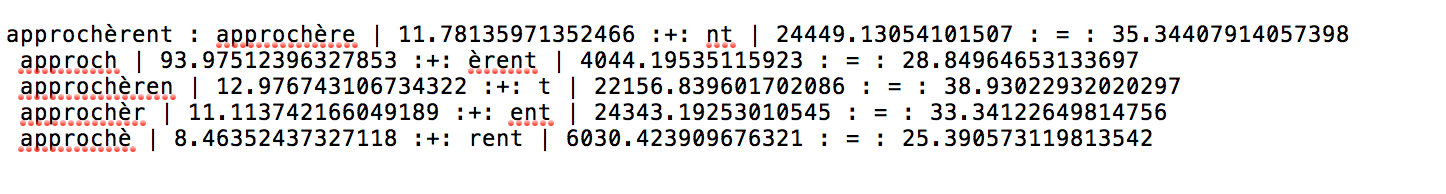
\includegraphics[width = 500pt]{seg_info.png}
\caption{Exemple de triplet de vraisemblances pour plusieurs segmentation du mot 'approchèrent'}
\end{figure}


En regardant ses résultats on se rend compte qu'on ne peut pas choisir une segmentation en ne triant que sur un seul indice. Pour parvenir à une unique segmentation nous appliquons l'arbre de décision suivant :

Si pour les maximums pour chacune des informations nous donnent une unique segmentation on utilise celle-là. \\
Si on obtient deux maximum menant à une segmentation alors on garde celle-ci. \\
Si toutes les segmentations sont différentes alors on prends celle donnée par le maximum d'information provenant des radicaux. 


Dans le cas de l'exemple ci-dessus on a : 
\begin{itemize}
\item Le maximum au sens des segmentations est : 'approchèren' + 't' \\ 
\item Le maximum au sens des suffixes est : 'approchèr' + 'ent' \\
\item Le maximum au sens des radicaux est : 'approch' + 'èrent' \\
\end{itemize}

Nous avons trois segmentations, on garde celle au sens des radicaux donc : 'approch' + 'èrent'. Nous avons désormais une unique segmentation pour chaque mot, on créer les signatures et on les sauvegarde
dans $"leftsig.txt"$ et $"rightsig.txt"$. 

Par exemple on obtient : 
\begin{figure}[!h]
\centering
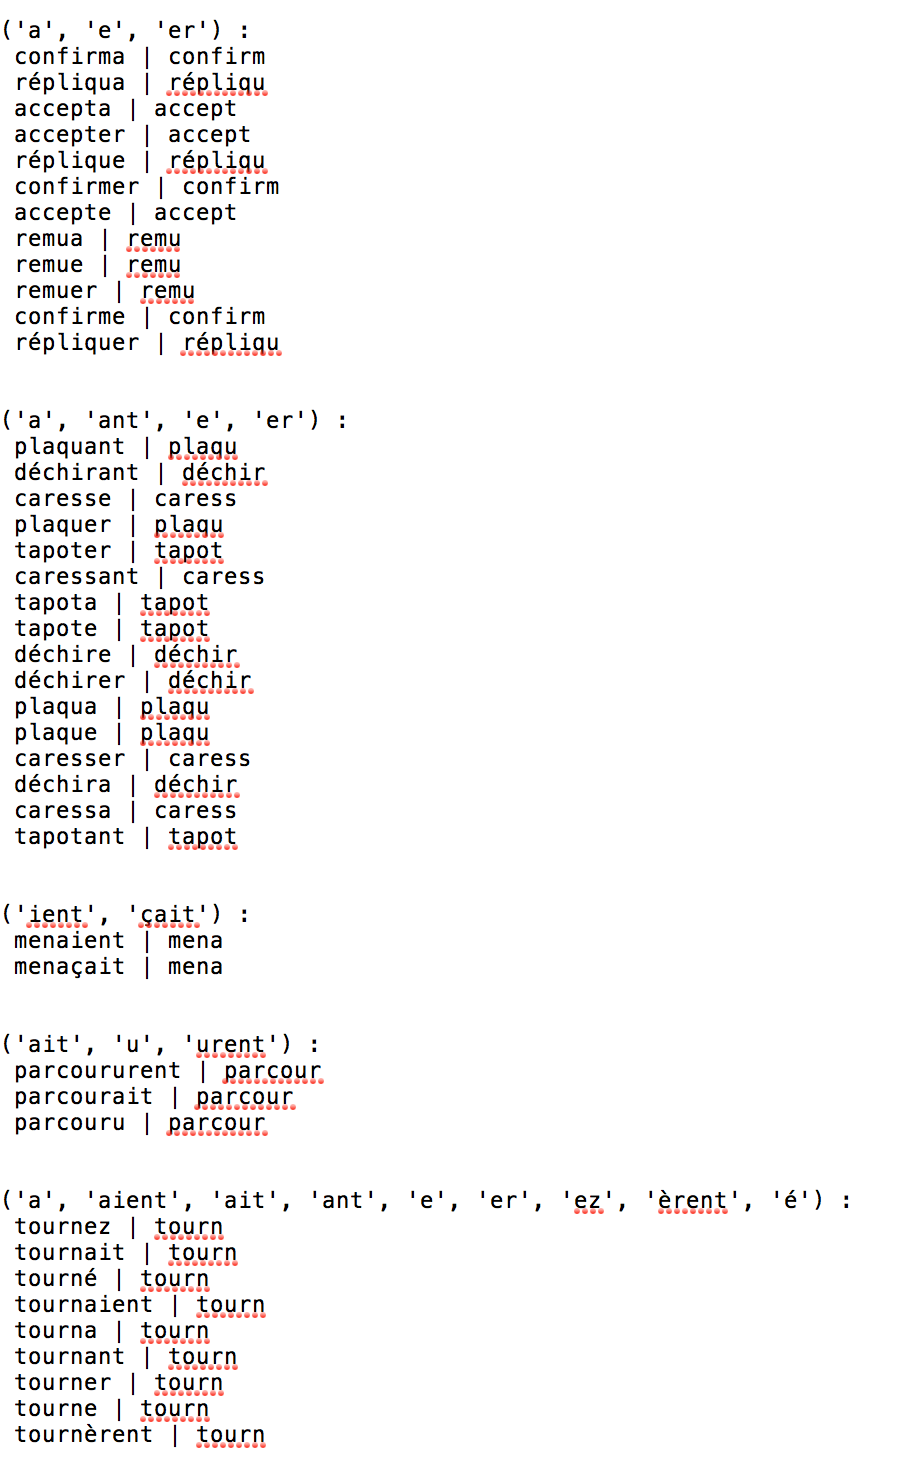
\includegraphics[width = 200pt]{example_sig.png}
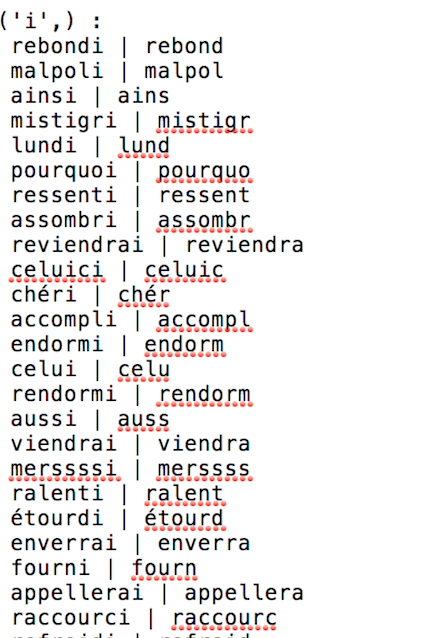
\includegraphics[width = 150pt]{example_sig3.png}
\end{figure}

\subsection{Résultats, critiques, comment continuer}


Plusieurs observations peuvent être faîtes sur la démarche effectuée. Contrairement à la méthode initialement prise (Goldsmith) celle-ci n'est pas non-supervisée. Quant aux résultats on observe trois choses.
\begin{itemize} 
\item La première est que dès lors qu'un verbe apparait sous beaucoup de formes dans le texte on est presque sûr de le retrouver seul dans une signature. ( Voir 'tournez', 'tournait', 'tournant' etc.... dans la photo ci-dessus).
\item La seconde est que au contraire on obtient des signatures ('s'), ('t') , qui vont prendre soit tous les noms qui apparaissent au pluriel ou les verbes qui n'apparaissent que dans peu de formes. 
\item La troisième est que l'on obtient quand même de bonnes signatures ( voir les deux premières sur la photo ci-dessus.)
\end{itemize}

Les deux premières correspondent, je pense, à des optimums locaux. La première parce que les signatures de cette forme ne contiennent généralement qu'un seul radical, qui est suivi de beaucoup de suffixes. Le radical a donc une 
grande vraisemblance et est gardé. La seconde parce que les signatures de cette forme ne contiennent généralement qu'un suffixe et pour les même raisons la segmentation et le suffixe auront une grande vraisemblance. Il faut aussi noter que dans la construction des suffixes la taille des suffixes que l'on créé dépends de la taille du mot. Plus le mot est long plus nous autorisons les suffixes long. De plus nous ne prenons pas en compte les mots de taille inférieur à 4. Sur les 8088 mots d'origine dans Harry Potter (en français) nous en étudions 7320. Nous obtenons au final 5149 radicaux différent et 348 suffixes différents. On peut penser qu'il serait judicieux de traiter les suffixes que l'on retrouve dans d'autres suffixes ('ons' et 'rons' par exemple) mais en faisant cela on risque de se retrouver avec seulement des suffixes à une lettre. Ce n'est pas ce que l'on veut.

Cette méthode est indépendante de la langue utilisée. En raison des hypothèses faites sur les tailles des suffixes cette méthode obtiendra de meilleurs résultats sur les langues indo-européennes et plus particulièrement pour les langues latines et l'anglais. L'allemand par exemple ou des mots juxtaposés peuvent former de nouveaux mots n'est pas adapté à cette méthode. 


\paragraph{Aller plus loin}

On se rend compte que l'étape primordiale est ici de trouver une bonne segmentation des mots. Les signatures se font ensuite très rapidement sans aucune autre hypothèse les segmentations trouvées. Pour cela, il y a une méthode que j'aurai voulu essayer si j'avais eu plus de temps. Il s'agit de celle défini par MATHIAS CREUTZ and KRISTA LAGUS dans leur article de \underline{Unsupervised Models for Morpheme Segmentation} \underline{and Morphology Learning} où il choisissent de maximiser la probabilité a posteriori de la segmentation. Si cette méthode me tente, c'est parce qu'elle est non-supervisée. Je souhaiterai aussi pouvoir implémenter un outil de segmentation d'un texte. Ces algorithmes visent à retrouver les mots dans un texte où les espaces ont été enlevés. Ceci nous permettrai de faire de l'alignement sur des langues comme le japonais ou le chinois.

 

















\end{document}  
  
